%
%----------------------------------------------------------------------------------------
%	PACKAGES AND OTHER DOCUMENT CONFIGURATIONS
%----------------------------------------------------------------------------------------
\documentclass{article}

\usepackage[left=2.5cm,right=2.5cm,top=2.5cm,bottom=2.5cm]{geometry}
\usepackage[centerlast,small,sc, margin=1cm]{caption}
\usepackage{subcaption}
\usepackage[round, square, numbers, comma, sort&compress]{natbib}
\usepackage[utf8]{inputenc}
\usepackage[nodayofweek]{datetime}
\usepackage{float}
\usepackage{graphicx}
%\usepackage[scriptsize]{subfigure}
\usepackage{pdfpages}
\usepackage{amsmath}
\usepackage{amsmath,amsfonts,amssymb,amscd,xspace}
\usepackage{afterpage}
\usepackage[pdfpagemode={UseOutlines},bookmarks=true,bookmarksopen=true,
   bookmarksopenlevel=0,bookmarksnumbered=true,hypertexnames=false,
   colorlinks,linkcolor={blue},citecolor={blue},urlcolor={red},
   pdfstartview={FitV},unicode,breaklinks=true]{hyperref}
%SRL
\usepackage{booktabs}

\hypersetup{urlcolor=blue, colorlinks=true}

\newcommand{\fref}[1]{Figure~\ref{#1}}

\newcounter{dummy}
\newcommand\addtotoc[1]{
\refstepcounter{dummy}
\addcontentsline{toc}{chapter}{#1}}

\graphicspath{{./Figures/}}
	
\makeatletter
\@fpsep\textheight
\makeatother

\begin{document}

%----------------------------------------------------------------------------------------
%	TITLE PAGE
%----------------------------------------------------------------------------------------

\title{Visualization of skeletal muscle based movement\\May Report}
\author{Moises Alencastre-Miranda \and Octavio Navarro-Hinojosa \and Sergio Ruiz Loza}
\date{\today}
\maketitle

%----------------------------------------------------------------------------------------
%	ABSTRACT PAGE
%----------------------------------------------------------------------------------------

%\addtotoc{Abstract} % Add the "Abstract" page entry to the Contents

\abstract{\addtocontents{toc}{\vspace{1em}}}

In order to obtain realistic animations, simulations and/or visualizations of muscle based movements, we want to generate a model based on Lattice Boltzmann and biophysical activation models, to best simulate how these work, and generate more realistic and accurate human movement animations and simulations. Here, we present the progress that has been achieved in different areas, including development of a Lattice Boltzmann solver in CUDA using Thrust, and development of a user interface to render and present the simulations of the proposed model.

%----------------------------------------------------------------------------------------
%	CONTENT - CHAPTERS
%----------------------------------------------------------------------------------------

% Include the chapters as separate files from the Chapters folder

\section{Introduction}
\label{Introduction}

\paragraph{}Human character’s animations and simulations are used in many fields: from video games and movies to robotic and medical simulations. Most of the animations of virtual human characters, the visualization or simulation of human movements, and many humanoid robot movements issues, are commonly solved assuming that the movement of each bone or extremity is produced in each joint, as if there were a motor in each one producing the movement. However, said approach does not simulate how real movement is generated, and does not produce realistic movements. In order to achieve more realistic movement, they  should be based on skeletal muscles.

\subsection{Skeletal Muscles}

\paragraph{}Skeletal muscles are among the most important structures in the human body. They are the most abundant tissue in the body (between 40\% and 45\% of the total body weight), they provide protection for internal tissues, they maintain the body's posture, and are a key component for force generation and movement. Skeletal muscle contraction is controlled through the somatic nervous system and, for the most part, is done so consciously. These voluntary contractions produce forces which transfer to the underlying skeleton, resulting in human body movement. 

\paragraph{}Each muscle is formed by two units: the muscle belly, and two tendinous units at each end of the muscle belly that connect it to the related bone. \fref{fig:muscleStructure} shows the hierarchical structure of the different tissues that compose a skeletal muscle. Skeletal muscles are wrapped by the episysium, a dense connective tissue which joins with the tendon. Internally, the muscle is composed of numerous muscle fiber bundles, called fascicles, which are separated from one another by a layer of connective tissue knowns as the perimysium. In turn, every fascicle consists of muscle fibers, which are isolated from one another by the endomysium. Muscle fibers are the structures that generate the contraction in a muscle. These are activated by  motor neurons that receive activation signals from the nervous system. Each motor neuron activates a group of fibers, and each group of fibers and motor neuron is called the motor unit.

\paragraph{}Another important component to be considered is tendon. It transmits forces produced by the attached muscle to bone. Tendon connects muscle to bone either at a narrow area or over a wide and flattened area, known as the aponeurosis. The attachment of muscle to more stationary bone (i.e., the proximal site) is called the origin while the other end to more movable bone (i.e., distal site) is called the insertion. Tendons are mostly composed of parallel arrays of collagen fibers closely packed together and have the mechanical property that they are much stiffer than muscles when they are pulled. In addition to force transmission, tendon has a function to passively modulate force during locomotion, providing additional stability \citep{oatis2009kynesiology, lee2010survey}. 

\afterpage{
\begin{figure}[t!]
	\centering
		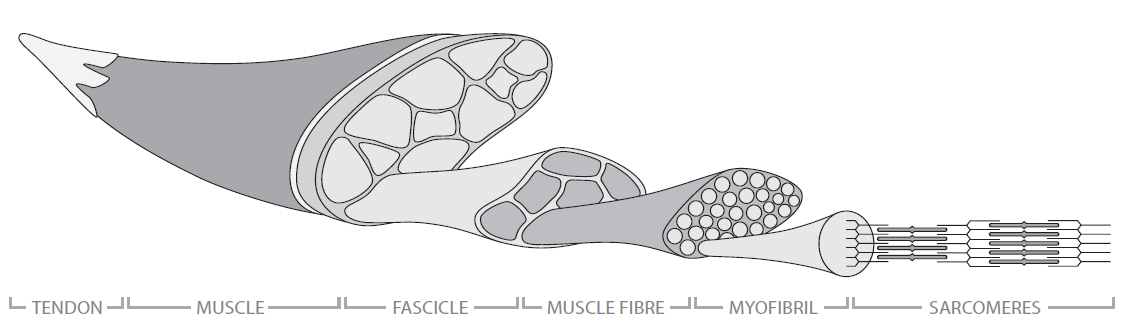
\includegraphics[scale=0.5]{muscleStructure.png}
	\caption{Major components of the muscle. Adapted from \citep{lee2010survey}.}
	\label{fig:muscleStructure}
\end{figure}
}

\subsection{Activation models}

\paragraph{}In order to simulate the muscle's contraction and generate force and movement, there are two main approaches: phenomenological and biophysical models \citep{tang20093d, rohrle2012physiologically}. Phenomenological models use mathematical and physics based constructs to describe the mechanical properties of biological tissue; in this case, skeletal muscles. One of the most used model is the Hill muscle model \citep{hill1970first}. This model is based on a series of experiments conducted on frog muscles, and captures the mechanical properties of the muscle. It has three major components: the series element (SE), the parallel element (PE), and the contractile element (CE). The series element (SE) represents mainly the elastic effects of tendon and intrinsic elasticity within the sarcomere. The parallel element (PE) represents the passive elasticity of the muscle resulting from the penetration of connective tissues into the muscle body. The contractile element (CE) accounts for generation of active force which is dependent on the muscle length, and the time-varying neural signal, a(t), originating from the central nervous system.

\paragraph{}On the contrary, biophysical models use physics to try to model biological systems. For muscle contraction, these models try to predict the muscle's response to a determinate stimulus. One commonly used biophysical model is the Huxley muscle contraction theory, that analyses the electrical activity of muscle fibers in order to generate movement. However, the Bidomain model \cite{rohrle2010simulating} is better suited at modelling the electric activity throughout a biological tissue. In the case of muscle contraction, based on a stimulus it calculates the muscle fiber's state before, during, and after a muscle contraction.

\subsection{State of the art}

\paragraph{}Since skeletal muscle are fundamental to maintain pose and to generate movement, there have been many studies that try to model the musculoskeletal system. For brevity, we will only mention the ones that have been relevant in the recent years.

\paragraph{}Lee and Terzopoulos \citep{lee2009comprehensive} developed a biomechanical model of the upper body. Their model is capable of modelling and controlling the muscles and bones, as well as simulating the physics-based deformations of the soft tissues. They incorporated 814 muscles, each of which is modeled as a piecewise uniaxial Hill-type force actuator. To simulate biomechanically-realistic flesh deformations, they developed a coupled finite element model with the appropriate constitutive behavior, in which are embedded the detailed 3D anatomical geometries of the hard and soft tissues. Finally, they created an associated physics-based animation controller that computes the muscle activation signals necessary to drive the elaborate musculoskeletal system in accordance with a sequence of target poses specified by an animator. A sample of their model can be seen in \fref{fig:muscleTorso}.

\afterpage{
\begin{figure}[t!]
	\centering
		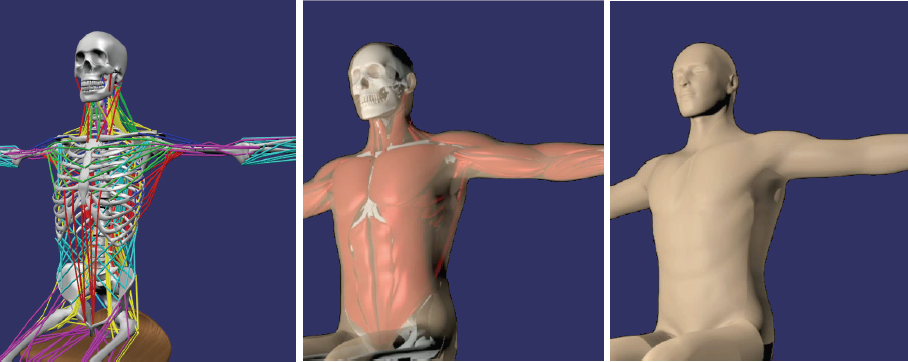
\includegraphics[scale=0.5]{muscleTorso.png}
	\caption{A skeleton moved by muscle modelled with a piecewise uniaxial Hill-type force actuator (left). The generated movement deforms the soft tissues (center), and the skin (right). Adapted from \citep{lee2009comprehensive}.}
	\label{fig:muscleTorso}
\end{figure}
}

\paragraph{}Unlike the work of Lee and Terzopoulos that use phenomenological models to generate force and movement, the work of Röhrle \citep{rohrle2010simulating, rohrle2012physiologically} uses the Bidomain model to describe the electrical activity and the subsequent contraction of the muscle fibers. The result is a physiologically based, multi-scale skeletal muscle finite element model that is capable of representing detailed, geometrical descriptions of skeletal muscle fibers and their grouping.

\paragraph{}Both previous works focus on a muscle model that has a physically based activation model, and use the Finite Element Method (FEM) to represent the muscle. The work of Fan et. al. \citep{fan2014active} focuses more on the visual accuracy rather than on the activation method. They introduce a framework for simulating the dynamics of musculoskeletal systems, with volumetric muscles in close contact and novel data-driven muscle activation model. Muscles are simulated using an Eulerian-on-Lagrangian discretization that handles volume preservation, large deformation, and close contact between adjacent tissues. Volume preservation is crucial for accurately capturing the dynamics of muscles and other biological tissues. Their model utilizes knowledge of the active shapes of muscles, which can be easily obtained from medical imaging data or designed to meet artistic needs. Their framework can be seen in \fref{fig:activeVolumetricMuscles}.

\afterpage{
\begin{figure}[t!]
	\centering
		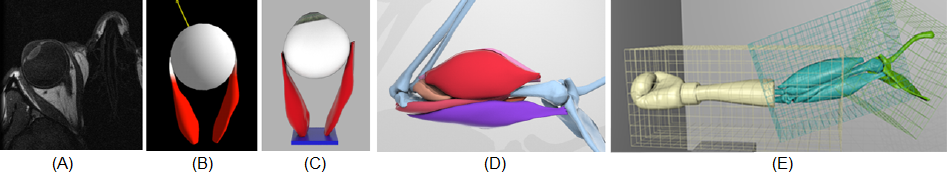
\includegraphics[keepaspectratio, scale=0.6]{activeVolumetricMuscles.png}
	\caption{The framework spans the entire pipeline for simulating volumetric musculoskeletal systems, starting from data on the active shapes of muscles to physically based simulation of muscles and soft tissues coupled to the skeletal system. The framework starts with muscle MRI data (A), then a reconstruction of the shape of the muscle is done in a 3D modelling software (B), and a simulation with the proposed method is generated (C). A set of six muscles of the arm are modelled (D), and those muscles are used in a dynamic simulation, with real bulging, tissue deformation, and contact with a simulated environment (E) \citep{fan2014active}.}
	\label{fig:activeVolumetricMuscles}
\end{figure}
}

\subsection{Problem statement}

\paragraph{}The musculoskeletal system consists of several biological structures, and is a crucial component for the analysis and simulation of human movement. However, it is inherently difficult to simulate this system, not just because of the complexity of the structures that conform it, but also because of all the relations between them that have to be taken into account.

\paragraph{}There are many challenges that have to be resolved in order to correctly simulate the musculoskeletal system. Some of them are as follows:

\begin{itemize}
	\item Most current simulations are simplifications of the overall system; either by simplifying the structures that the model uses, or the way they are controlled.  
	\item The way in which the tissues are simulated not always accounts for certain key properties, such as volume conservation, or bulging; or are simulated using techniques such as FEM, that are computationally expensive, and more so if such properties are to be considered.
	\item Most previous work does not model the muscle fibers, which are crucial for a correct muscle simulation.
	\item The mainly used activation methods are phenomenological. These are simplifications of the real behaviour of muscles, and have been proven to be wrong when comparing their output to real muscle output data. These models are more similar to simple mechanic systems than to biological systems. 
	\item The physical properties of the several components of the musculoskeletal system are normally not taken into account.
	\item Bones, ligaments, and tendons are either simplified or ignored for most simulations. 
\end{itemize}

\paragraph{}Currently, there does not exist a model of the musculoskeletal system that simulates the muscles considering their internal structure, the biological tissues that they are composed of, and their physical and biological properties, that is also activated using biophysical models that emulate how they respond to a signal from the nervous system. Additionally, most previous work focus on modelling a specific muscle, or a group of specific muscles, without providing a framework that can help model any muscle of the body.

\paragraph{}Furthermore, the computational cost to solve the different mathematical, and physical models, as well as the rendering of the various objects in the scene, can be high. However, not many studies rely on General Purpose computing on Graphics Processing Units (GPGPU), making their solutions not ideal for interactive or real time simulations.

\subsection{Proposed method}

\paragraph{}In order to try to solve many of the issues presented, we propose a solution that involves several techniques that have been shown to produce more correct results when it comes to model the musculoskeletal system. 

\paragraph{}The first issue that needs to be solved is the simplification of the musculoskeletal system. We propose a model that encompasses several of the principal tissues and structures that are present in every muscle: the muscle fibers, connecting tissues, tendons, bone, and skin. Since the human body is comprised mostly of water, most of these tissues could be modelled using computational fluid dynamics (CFD) methods for fluid simulation. In this case, we propose the use of a modified Lattice Boltzmann Method (LBM) to model all the mentioned tissues. 

\paragraph{}Normally, LBM models the flow of a fluid within a container. For this solution, the fluids are going to be the tissues of the body, each with their own material properties; and unlike normal LBM simulations, where each element of the lattice has a related density and speed distribution that dictates the flow of the fluid, we will use said speeds and material properties to simulate a very viscous, almost solid fluid, that modifies its container when needed (such as when an external force is present). This allows the tissue to have basic biological properties, such as being deformable, incompressible, having volume preservation, and allowing the contact with other tissues.

\paragraph{}The proposed simulation of tissues requires the use of a very detailed human 3D model. We propose the use of The Visible Human Project model \citep{visibleHumanProject} from the 















\section{Lattice Boltzmann Solver}
\label{LBS}

\paragraph{}Lattice Boltzmann models (LBM) is a class of computational fluid dynamics (CFD) methods for fluid simulation. Instead of solving the Navier–Stokes equations, the discrete Boltzmann equation is solved to simulate the flow of a Newtonian fluid with collision models such as Bhatnagar-Gross-Krook (BGK). By simulating streaming and collision processes across a limited number of particles, the intrinsic particle interactions create a flow behavior applicable across an entire lattice.

\paragraph{}Lattice Gas Cellular Automaton (LGCA) models were the harbingers of LBM. LGCA were presented as a viable means of solving the Navier-Stokes equations of fluid motion. Ludwig Boltzmann used these models to introduce the Boltzmann Gas Concept, where the idea is that a gas is composed of interacting particles that can be described by classical mechanics, and, because there are so many particles, a statistical treatment is necessary and appropriate. The mechanics can be extremely simple and encapsulated by just
the notions of streaming in space and billiard-like collision interactions.

\paragraph{}LBM vastly simplify Boltzmann’s original conceptual view by reducing the number of possible particle spatial positions and microscopic momenta from a continuum to just a handful and similarly discretizing time into distinct steps. Particle positions are confined to the nodes of the lattice. Variations in momenta that could have been due to a continuum of velocity directions and magnitudes and varying particle mass are reduced (in the simple 2-D model we focus on here) to 8 directions, 3 magnitudes, and a single particle mass \citep{sukop2006lattice}. \fref{fig:d2q9} shows the Cartesian lattice and the velocities $e_a$ where a = 0, 1, \dots , 8 is a direction index and $e_0$ = 0 denotes particles at rest. This model is known as D2Q9 as it is 2 dimensional and contains 9 velocities.

\begin{figure}[t!]
	\centering
		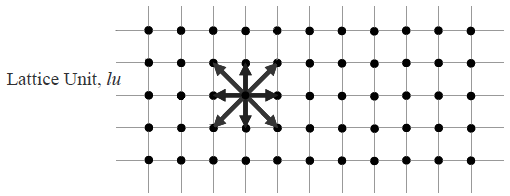
\includegraphics[scale=0.7]{d2q9.png}
	\caption{D2Q9 lattice and velocities. Adapted from \citep{sukop2006lattice}.}
	\label{fig:d2q9}
\end{figure}

Because particle mass is uniform (1 mass unit or mu in the simplest approach), these microscopic velocities and momenta are always effectively equivalent. The lattice unit (lu) is the fundamental measure of length in the LBM models and time steps (ts) are the time unit. 

The velocity magnitude of $e_1$ through $e_4$ is 1 lattice unit per time step or 1 lu ${ts}^{-1}$, and the velocity magnitude of $e_5$ through $e_8$ is $\sqrt{2}$ lu ${ts}^{-1}$. (While this is probably the most common velocity indexing scheme, be aware that others are in use.) These velocities are exceptionally convenient in that all of their $x$ and $y$ components are either $0$ or $\pm 1$.

\section{Muscle Visualization Module}
In order to test, evaluate and later validate the proposed method, we started the development of a visualization software tool that is able to display geometry efficiently by using parallel hardware (GPU) techniques; the visualization software will also provide an interface to control simulation parameters.

%----------------------------------------------------------------------------------------

\subsection{Visualization Implementation}

By using a set of third party software tools, we assembled a rendering engine (Figure~\ref{fig:muscleVis}) that allows efficient display and control of a simulation that uses the proposed method. Open Source libraries for rendering, shading, graphical user interface, texture and geometry loading have been integrated to the visualization software; these tools are listed in Table~\ref{tab:thirdSw}.

\begin{figure}[!t]
	\centering
		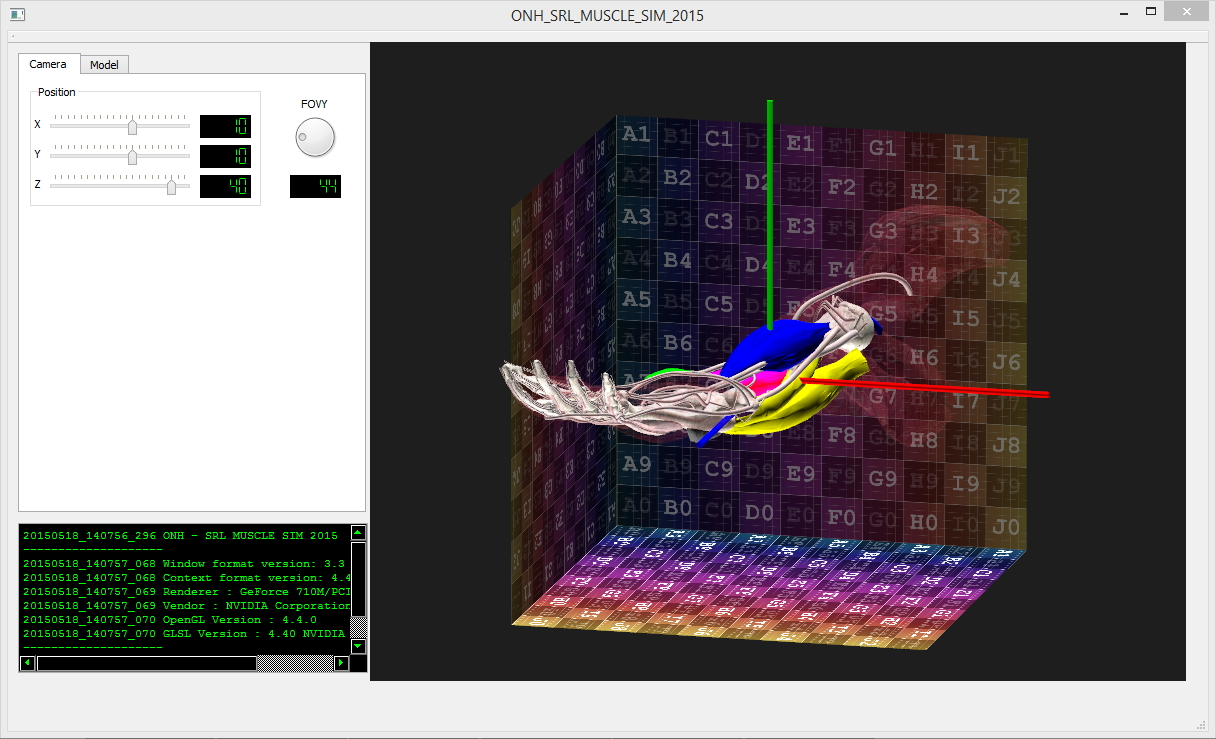
\includegraphics[width=0.8\textwidth]{./Figures/viewConfig.jpg}
	\caption[Muscle rendering.]{Muscle rendering tool.}
	\label{fig:muscleVis}
\end{figure}

\begin{table}[htbp]
  \centering
  \caption{Third party software for virtual muscle rendering}
    \begin{tabular}{rr}
    \toprule
    \multicolumn{2}{c}{\textbf{Third party software tools}} \\
    \midrule
    \textbf{Rendering Library} & OpenGL \\
    \textbf{Shading} & GLSL \\
    \textbf{GUI} & Qt 5.4.1 Community \\
    \textbf{Texture loader} & DevIL \\
    \textbf{Geometry loader} & ASSIMP \\
    \bottomrule
    \end{tabular}%
  \label{tab:thirdSw}%
\end{table}%

\subsection{Rendering Advances}

From the BodyParts3d~\citep{bodyParts3d} database, we have identified, colored and separated virtual muscle geometries (Figure~\ref{fig:muscleView}) of interest\textemdash right biceps brachii, brachialis, brachiordialis, pronator teres, triceps brachii, anconeus\textemdash that will serve as input for the muscle simulation. Together, all the arm meshes are composed of 271,004 faces which are rendered at interactive frame rates: up to 0.00588235 seconds per frame using a Nvidia GeForce 710M GPU as shown in Figure~\ref{fig:muscleRendering}, thus allowing for simulation computations to be performed even on the same hardware.

\begin{figure}[t]
    \centering
    \begin{subfigure}[t]{0.45\textwidth}
        \centering
        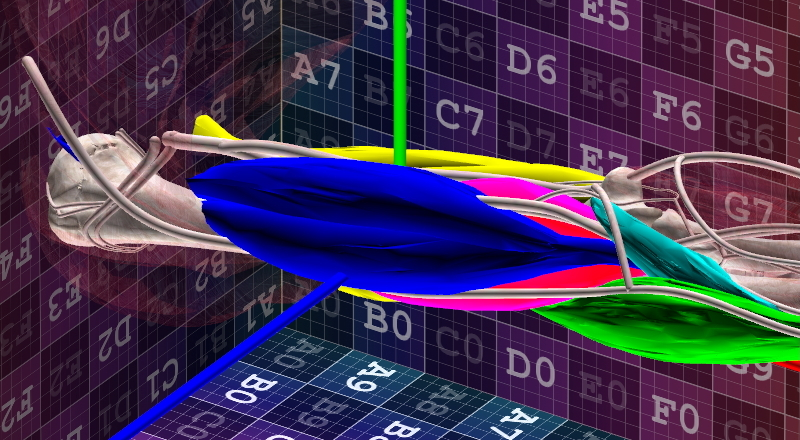
\includegraphics[width=\textwidth]{./Figures/musclesFront.jpg}
        \caption{Blue: biceps brachii. Purple: brachialis. Green: brachiordialis. Aqua: pronator teres.}
        \label{fig:musclesFront}
    \end{subfigure}
\hfill
    \begin{subfigure}[t]{0.45\textwidth}
        \centering
        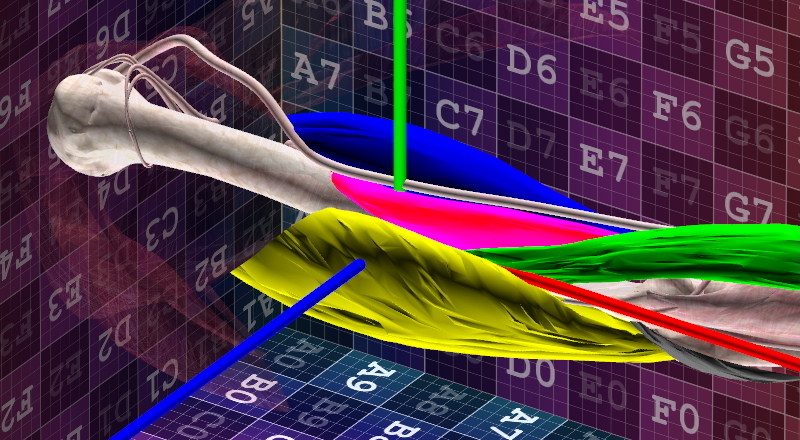
\includegraphics[width=\textwidth]{./Figures/musclesBack.jpg}
        \caption{Yellow: triceps brachii. Gray: anconeus.}
        \label{fig:musclesBack}
    \end{subfigure}

    \caption{Muscle geometry}
    \label{fig:muscleView}
\end{figure}

\afterpage{
\begin{figure}[t]
    \centering
    \begin{subfigure}[t]{0.45\textwidth}
        \centering
        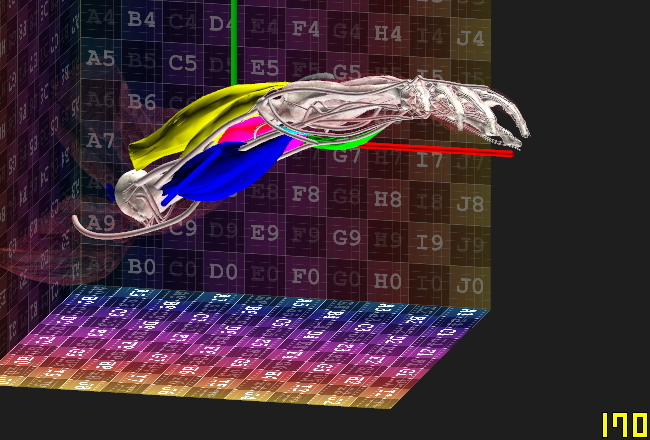
\includegraphics[width=\textwidth]{./Figures/visFPS.jpg}
        \caption{Interactive rate rendering.}
        \label{fig:visFPS}
    \end{subfigure}
	\hfill
    \begin{subfigure}[t]{0.45\textwidth}
        \centering
        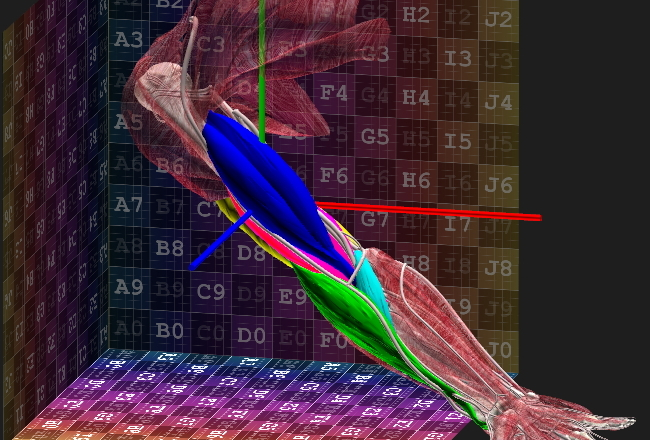
\includegraphics[width=\textwidth]{./Figures/transparencyConfig.jpg}
        \caption{Transparency control.}
        \label{fig:transparency}
    \end{subfigure}

    \caption{Muscle rendering}
    \label{fig:muscleRendering}
\end{figure}
}
%\begin{figure}
%    \centering
%    \begin{subfigure}[t]{0.45\textwidth}
%        \centering
%        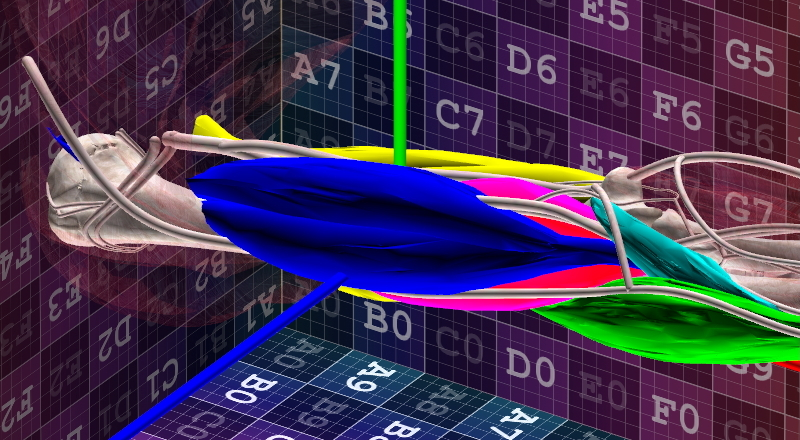
\includegraphics[width=\textwidth]{./Figures/musclesFront.jpg}
%        \caption{Blue: biceps brachii. Purple: brachialis. Green: brachiordialis. Aqua: pronator teres.}
%        \label{fig:musclesFront}
%    \end{subfigure}
%\hfill
%    \begin{subfigure}[t]{0.45\textwidth}
%        \centering
%        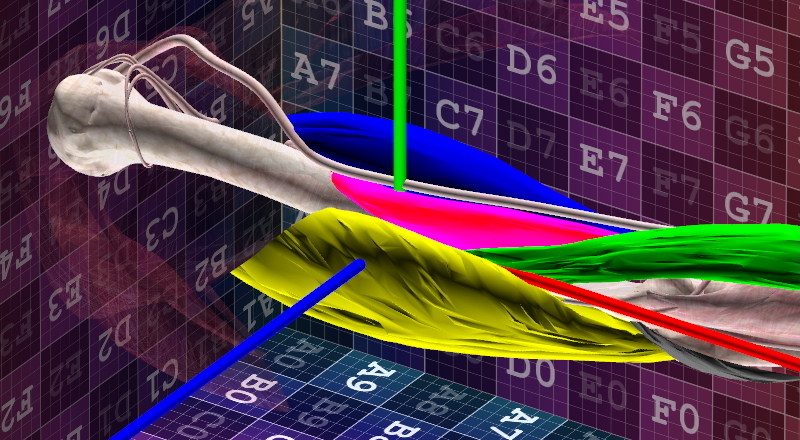
\includegraphics[width=\textwidth]{./Figures/musclesBack.jpg}
%        \caption{Yellow: triceps brachii. Gray: anconeus.}
%        \label{fig:musclesBack}
%    \end{subfigure}
%
%    \caption{Muscle geometry}
%    \label{fig:muscleView}
%\end{figure}
%
%
%\begin{figure}
%    \centering
%    \begin{subfigure}[t]{0.45\textwidth}
%        \centering
%        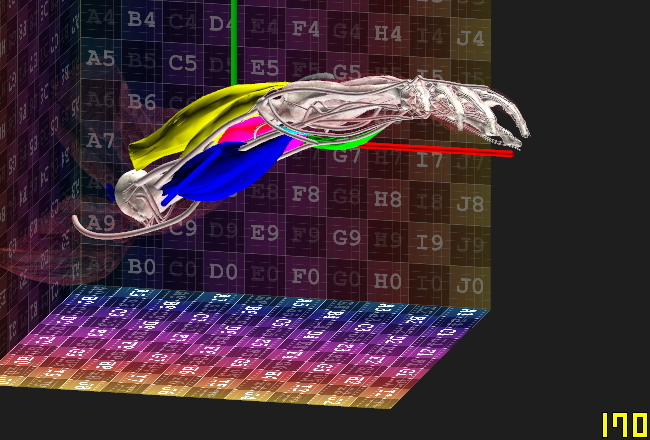
\includegraphics[width=\textwidth]{./Figures/visFPS.jpg}
%        \caption{Interactive rate rendering.}
%        \label{fig:visFPS}
%    \end{subfigure}
%	\hfill
%    \begin{subfigure}[t]{0.45\textwidth}
%        \centering
%        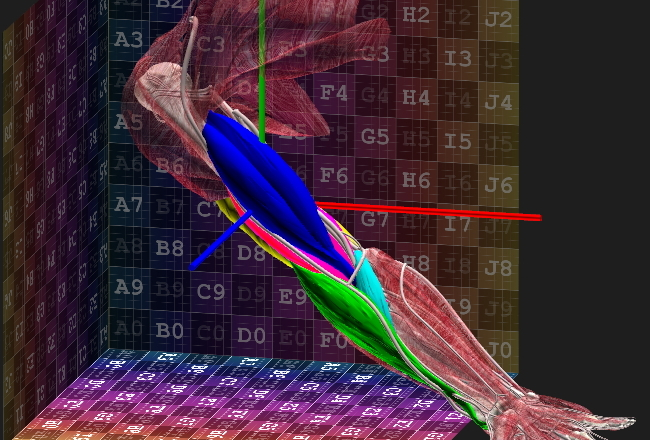
\includegraphics[width=\textwidth]{./Figures/transparencyConfig.jpg}
%        \caption{Transparency control.}
%        \label{fig:transparency}
%    \end{subfigure}
%
%    \caption{Muscle rendering}
%    \label{fig:muscleRendering}
%\end{figure}

\section{Future Work}
\label{sec:futureWork}
In addition to the Lattice Boltzmann Solver and Visualization integration, we have identified several future work opportunities:

\begin{description}
\item[Octrees]
Vertex identification as part of a simulated muscle will be efficient by means of a specialized data structure. We will integrate the Point Cloud Library (PCL) to our rendering engine making use of its parallel octree implementation.
\item[Level of Detail]
As computational resources become scarce due to real-time simulation and rendering requirements, implementation of a Level of Detail technique will improve hardware performance.
\item[Clipping]
Sections of a virtual extended arm will be useful to calculate intermuscular space from different poses, as an extension of the muscular simulation.
\item[Simulation control]
LBM simulations require fine tuning of viscosity and grid size parameters. Future work will extend the user interface to facilitate parameter adjustment in real-time.
\item[Bidomain Fiber simulation]
We will implement a fiber simulation and rendering as the basic activation unit for our model, based on the Bidomain simulation. Bidomain Fiber simulation force will be the input to the LBM mesh deformation algorithm.
\item[Inter mesh Collision]
In future work we will solve intermuscular collision and tension forces, adding precision to the muscle simulation.
\item[Muscle-Bone Hierarchy]
For animation, we will establish not only the bone rigging hierarchy, but also the various insertion points for tendons, achieving precise physics-based simulations activated by the Bidomain-LBM algorithm.
\item[Kernel configuration]
We will test further Kernel (grid/block/trhead) launch configurations as well as other LBM models to ensure optimal algorithm performance. 
\end{description}


%----------------------------------------------------------------------------------------
%	BIBLIOGRAPHY
%----------------------------------------------------------------------------------------

\label{Bibliography}

\addtotoc{Bibliography}
\addtocontents{toc}{\vspace{2em}}
\bibliographystyle{unsrtnat}
\bibliography{Bibliography} 

\end{document}  
